% This is a Basic Assignment Paper but with like Code and stuff allowed in it, there is also url, hyperlinks from contents included. 

\documentclass[11pt]{article}

% Preamble

\usepackage[margin=1in]{geometry}
\usepackage{amsfonts, amsmath, amssymb}
\usepackage{fancyhdr, float, graphicx}
\usepackage[utf8]{inputenc} % Required for inputting international characters
\usepackage[T1]{fontenc} % Output font encoding for international characters
\usepackage{fouriernc} % Use the New Century Schoolbook font
\usepackage[nottoc, notlot, notlof]{tocbibind}
\usepackage{listings}
\usepackage{xcolor}
\usepackage{blindtext}
\usepackage{hyperref}
\hypersetup{
    colorlinks=true,
    linkcolor=black,
    filecolor=magenta,      
    urlcolor=cyan,
    pdfpagemode=FullScreen,
    }

\definecolor{codegreen}{rgb}{0,0.6,0}
\definecolor{codegray}{rgb}{0.5,0.5,0.5}
\definecolor{codepurple}{rgb}{0.58,0,0.82}
\definecolor{backcolour}{rgb}{0.95,0.95,0.92}

\lstdefinestyle{mystyle}{
    backgroundcolor=\color{backcolour},   
    commentstyle=\color{codegreen},
    keywordstyle=\color{magenta},
    numberstyle=\tiny\color{codegray},
    stringstyle=\color{codepurple},
    basicstyle=\ttfamily\footnotesize,
    breakatwhitespace=false,         
    breaklines=true,                 
    captionpos=b,                    
    keepspaces=true,                 
    numbers=left,                    
    numbersep=5pt,                  
    showspaces=false,                
    showstringspaces=false,
    showtabs=false,                  
    tabsize=2
}

\lstset{style=mystyle}

% Header and Footer
\pagestyle{fancy}
\fancyhead{}
\fancyfoot{}
\fancyhead[L]{\textit{\Large{Information and Cycbersecurity - 2nd Year B. Tech}}}
%\fancyhead[R]{\textit{something}}
\fancyfoot[C]{\thepage}
\renewcommand{\footrulewidth}{1pt}



% Other Doc Editing
% \parindent 0ex
%\renewcommand{\baselinestretch}{1.5}

\begin{document}

\begin{titlepage}
	\centering

	%---------------------------NAMES-------------------------------

	\huge\textsc{
		MIT World Peace University
	}\\

	\vspace{0.75\baselineskip} % space after Uni Name

	\LARGE{
		Information and Cybersecurity\\
		Second Year B. Tech, Semester 1
	}

	\vfill % space after Sub Name

	%--------------------------TITLE-------------------------------

	\rule{\textwidth}{1.6pt}\vspace*{-\baselineskip}\vspace*{2pt}
	\rule{\textwidth}{0.6pt}
	\vspace{0.75\baselineskip} % Whitespace above the title



	\huge{\textsc{
			Classical Cryptographic Techniques - \\
			\textit{"Fiestal Cipher"}
		}} \\



	\vspace{0.5\baselineskip} % Whitespace below the title
	\rule{\textwidth}{0.6pt}\vspace*{-\baselineskip}\vspace*{2.8pt}
	\rule{\textwidth}{1.6pt}

	\vspace{1\baselineskip} % Whitespace after the title block

	%--------------------------SUBTITLE --------------------------	

	\LARGE\textsc{
		Lab Assignment 2
	} % Subtitle or further description
	\vfill

	%--------------------------AUTHOR-------------------------------

	Prepared By
	\vspace{0.5\baselineskip} % Whitespace before the editors

	\Large{
		Krishnaraj Thadesar \\
		Cyber Security and Forensics\\
		Batch A1, PA 20
	}


	\vspace{0.5\baselineskip} % Whitespace below the editor list
	\today

\end{titlepage}


\tableofcontents
\thispagestyle{empty}
\clearpage

\setcounter{page}{1}

\section{Aim}
Write a program using JAVA or Python or C++ to implement Feistal Cipher structure

\section{Objectives}
To understand the concepts of symmetric key cryptographic system.

\section{Theory}
\subsection{Symmetric Key Cryptography}

Symmetric key cryptography is a cryptographic system in which the same key is used for both encryption and decryption. The key is shared between the sender and the receiver. The sender encrypts the message using the key and sends it to the receiver. The receiver decrypts the message using the same key. The key is kept secret and is never sent along with the message.

The most commonly used symmetric key algorithm is the Data Encryption Standard (DES). It uses a 64-bit block size and a 56-bit key. The 64-bit block is divided into two halves of 32-bits each. The key is also divided into two halves of 28-bits each. The first half of the key is used to generate 16 subkeys. Each subkey is 48-bits long. The first 28-bits of the key are shifted left by 1 bit. The first 28-bits of the key are then shifted left by 1 bit. The second 28-bits of the key are shifted left by 1 bit. The second 28-bits of the key are shifted left by 1 bit. This process is repeated for the remaining 16 rounds. The 16 subkeys are then used to encrypt the message.

\subsection{Feistal Cipher}

Feistel Cipher model is a structure or a design used to develop many block ciphers such as DES. Feistel cipher may have invertible, non-invertible and self invertible components in its design. Same encryption as well as decryption algorithm is used. A separate key is used for each round. However same round keys are used for encryption as well as decryption.

\subsection{Fiestal Cipher Algorithm}

\begin{enumerate}
	\item Create a list of all the Plain Text characters.

	\item Convert the Plain Text to Ascii and then 8-bit binary format.

	\item Divide the binary Plain Text string into two halves: left half (L1) and right half (R1)

	\item Generate a random binary keys (K1 and K2) of length equal to the half the length of the Plain Text for the two rounds.

\end{enumerate}

\begin{figure}[H]
	\centering
	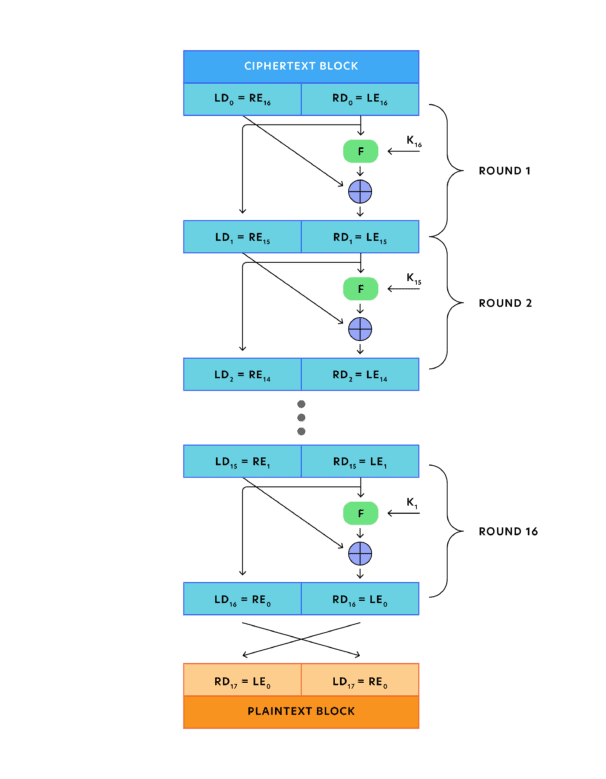
\includegraphics[scale=0.5]{fiestal_cipher.png}
	\caption{Fiestal Cipher Decryption Method}
\end{figure}


\section{Platform}
\textbf{Operating System}: Arch Linux x86-64 \\
\textbf{IDEs or Text Editors Used}: Visual Studio Code\\
\textbf{Compilers or Interpreters} : Python 3.10.1\\

\section{Input and Output}
\begin{verbatim}
    The plain text, key
    [1, 1, 1, 1, 0, 0, 1, 1] [1, 0, 1, 0, 0, 0, 0, 0, 1, 0]
    The left and right keys are :  [1, 0, 1, 0, 0, 1, 0, 0] [0, 1, 0, 0, 0, 0, 1, 1]
    Starting to cipher. 
    The cipher text is :  [0, 1, 0, 0, 0, 0, 0, 1]
\end{verbatim}
\section{Code}
\lstinputlisting[language=Python, caption="Fiestal Cipher"]{../Programs/Assignment_2/fiestel_cipher.py}

\section{Conclusion}
Thus, learnt about the different kinds of ciphers, classical cryptographic techniques, and how to implement some of them in python.
\clearpage

\section{FAQ}

\begin{enumerate}
	\item \textbf{Differentiate between stream and block ciphers.}\\
	      \begin{enumerate}
		      \item Stream ciphers encrypt the data one bit at a time. Block ciphers encrypt the data in blocks of fixed size.
		      \item Stream ciphers are faster than block ciphers.
		      \item Block ciphers are more secure than stream ciphers.
		      \item Stream ciphers are more suitable for real-time applications.
		      \item Block ciphers are more suitable for bulk data encryption.
		      \item Stream ciphers are more suitable for applications where the data is encrypted and decrypted in a single pass.
		      \item Block ciphers are more suitable for applications where the data is encrypted and decrypted in multiple passes.
	      \end{enumerate}

	\item \textbf{Write advantages and disadvantages of DES algorithm.}\\

	      \textbf{Advantages:}
	      \begin{enumerate}
		      \item It is a fast, simple, efficient, and secure algorithm.
		      \item The algorithm has been in use since 1977. Technically, no weaknesses have been found in the algorithm. Brute force attacks are still the most efficient attacks against the DES algorithm.
		      \item DES is the standard set by the US Government. The government recertifies DES every five years, and has to ask for its replacement if the need arises.
		      \item The American National Standards Institute (ANSI) and International Organization for Standardization (ISO) have declared DES as a standard as well. This means that the algorithm is open to the public—to learn and implement.
		      \item DES was designed for hardware; it is fast in hardware, but only relatively fast in software.
	      \end{enumerate}

	      \textbf{Disadvantages:}
	      \begin{enumerate}
		      \item Probably the biggest disadvantage of the DES algorithm is the key size of 56-bit. There are chips available that can encrypt and decrypt a million DES operations in a second. A DES cracking machine that can search all the keys in about seven hours is available for 1 million.
		      \item DES can be implemented quickly on hardware. But since it was not designed for software, it is relatively slow on it.
		      \item It has become easier to break the encrypted code in DES as the technology is steadily improving. Nowadays, AES is preferred over DES.
		      \item DES uses a single key for encryption as well as decryption as it is a type of symmetric encryption technique. In case that one key is lost, we will not be able to receive decipherable data at all.
	      \end{enumerate}

	\item \textbf{Explain block cipher modes of operations.}\\
	      \begin{enumerate}
		      \item \textit{Electronic Code Book (ECB)}
		            \begin{enumerate}
			            \item ECB mode stands for Electronic Code Block Mode. It is one of the simplest modes of operation. In this mode, the plain text is divided into a block where each block is 64 bits. Then each block is encrypted separately. The same key is used for the encryption of all blocks. Each block is encrypted using the key and makes the block of ciphertext.
			            \item At the receiver side, the data is divided into a block, each of 64 bits. The same key which is used for encryption is used for decryption. It takes the 64-bit ciphertext and, by using the key convert the ciphertext into plain text.
			            \item As the same key is used for all blocks’ encryption, if the block of plain text is repeated in the original message, then the ciphertext’s corresponding block will also repeat. As the same key used for tor all block, to avoid the repetition of block ECB mode is used for an only small message where the repetition of the plain text block is less.
		            \end{enumerate}

		            \begin{figure}[H]
			            \centering
			            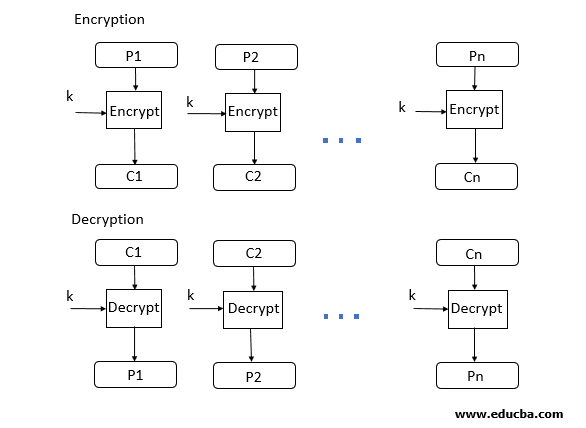
\includegraphics[scale=0.5]{ecb.jpg}
			            \caption{ECB Mode of Operation}
		            \end{figure}

		      \item \textit{Cipher Block Chaining (CBC)}
		            \begin{enumerate}
			            \item CBC Mode stands for Cipher block Mode at the sender side; the plain text is divided into blocks. In this mode, IV(Initialization Vector) is used, which can be a random block of text. IV is used to make the ciphertext of each block unique.
			            \item The first block of plain text and IV is combined using the XOR operation and then encrypted the resultant message using the key and form the first block of ciphertext. The first block of ciphertext is used as IV for the second block of plain text. The same procedure will be followed for all blocks of plain text.
			            \item At the receiver side, the ciphertext is divided into blocks. The first block ciphertext is decrypted using the same key, which is used for encryption. The decrypted result will be XOR with the IV and form the first block of plain text. The second block of ciphertext is also decrypted using the same key, and the result of the decryption will be XOR with the first block of ciphertext and form the second block of plain text. The same procedure is used for all the blocks.
			            \item CBC Mode ensures that if the block of plain text is repeated in the original message, it will produce a different ciphertext for corresponding blocks.
			                  Note that the key which is used in CBC mode is the same; only the IV is different, which is initialized at a starting point.
		            \end{enumerate}

		            \begin{figure}[H]
			            \centering
			            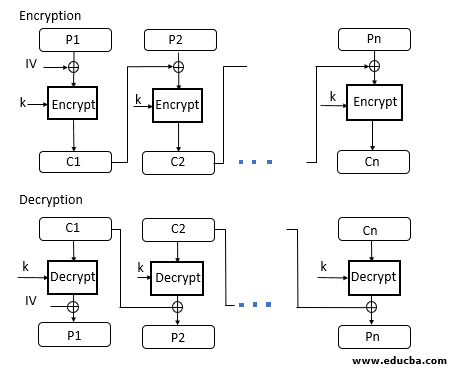
\includegraphics[scale=0.5]{cbc.jpg}
			            \caption{CBC Mode of Operation}
		            \end{figure}
		      \item \textit{Cipher Feedback (CFB)}

		            \begin{enumerate}
			            \item CFB mode stands for Cipher Feedback Mode. In this mode, the data is encrypted in the form of units where each unit is of 8 bits.
			            \item Like cipher block chaining mode, IV is initialized. The IV is kept in the shift register. It is encrypted using the key and form the ciphertext.
			            \item Now the leftmost j bits of the encrypted IV is XOR with the plain text’s first j bits. This process will form the first part of the ciphertext, and this ciphertext will be transmitted to the receiver.
			            \item Now the bits of IV is shifted left by j bit. Therefore the rightmost j position of the shift register now has unpredictable data. These rightmost j positions are now filed with the ciphertext. The process will be repeated for all plain text units.
		            \end{enumerate}

		            \begin{figure}[H]
			            \centering
			            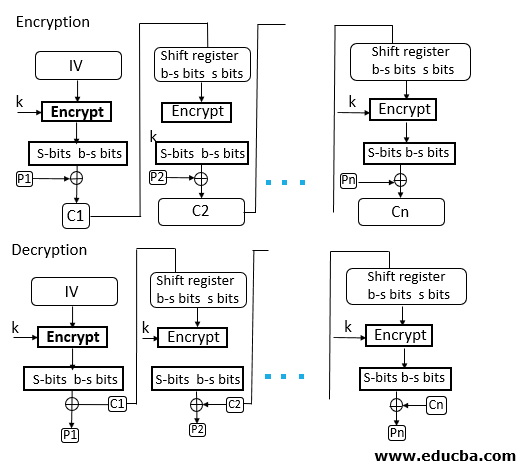
\includegraphics[scale=0.6]{cfb.jpg}
			            \caption{CFB Mode of Operation}
		            \end{figure}

		      \item \textit{Output Feedback (OFB)}

		            \begin{enumerate}
			            \item OFB Mode stands for output feedback Mode. OFB mode is similar to CFB mode; the only difference is in CFB, the ciphertext is used for the next stage of the encryption process, whereas in OFB, the output of the IV encryption is used for the next stage of the encryption process.
			            \item The IV is encrypted using the key and form encrypted IV. Plain text and leftmost 8 bits of encrypted IV are combined using XOR and produce the ciphertext.
			            \item For the next stage, the ciphertext, which is the form in the previous stage, is used as an IV for the next iteration. The same procedure is followed for all blocks.
		            \end{enumerate}

		            \begin{figure}[H]
			            \centering
			            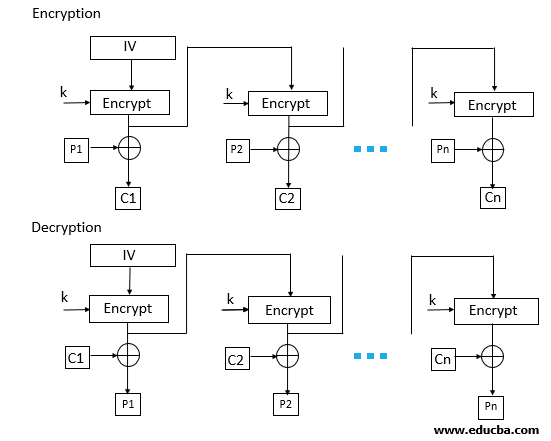
\includegraphics[scale=0.5]{ofm.jpg}
			            \caption{Output Feedback Mode of Operation}
		            \end{figure}
		      \item \textit{Counter (CTR)}

		            \begin{enumerate}
			            \item CTR Mode stands for counter mode. As the name is counter, it uses the sequence of numbers as an input for the algorithm. When the block is encrypted, to fill the next register next counter value is used.
			            \item For encryption, the first counter is encrypted using a key, and then the plain text is XOR with the encrypted result to form the ciphertext.
			            \item The counter will be incremented by 1 for the next stage, and the same procedure will be followed for all blocks. For decryption, the same sequence will be used. Here to convert ciphertext into plain text, each ciphertext is XOR with the encrypted counter. For the next stage, the counter will be incremented by the same will be repeated for all Ciphertext blocks.
		            \end{enumerate}

		            \begin{figure}[H]
			            \centering
			            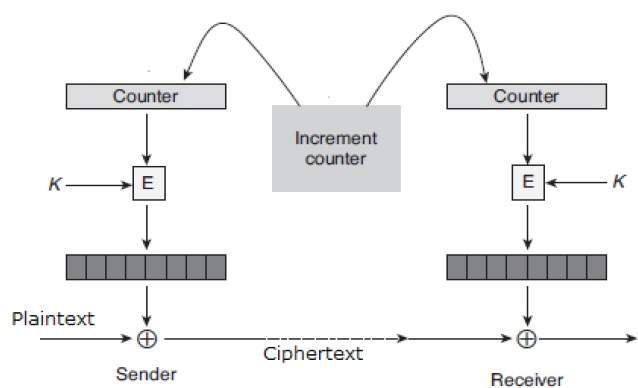
\includegraphics[scale=0.5]{ctr_mode.jpg}
			            \caption{}
		            \end{figure}
	      \end{enumerate}
\end{enumerate}

\end{document}